\chapter{La trave}

\section{Intoduzione}
\lipsum[1]

\section{Le caratteristiche della sollecitazione}
Le tensioni che agiscono sulla generica sezione trasversale della trave $\Tc=\Sc \times (0,\ell)$  sono

\begin{equation}
\tb=\Tb\eb_3=T_{13}\eb_1+T_{23}\eb_2+T_{33}\eb_3.
\end{equation}

Definiamo il risultante   delle azioni interne che agiscono sulla sezione trasversale
\begin{equation}\label{f}
\fb(x_3)\coloneqq\int_{\Sc}\tb (x_1, x_2, x_3)
\end{equation}
e il momento risultante delle stesse azioni rispetto al polo $(0,0,z)$:
\begin{equation}
\mb(x_3)\coloneqq\int_{\Sc}\pb(x_1,x_2) \times \tb(x_1, x_2, x_3).
\end{equation}
Indichiamo componenti di $\fb$ con 
\begin{definition}
	\begin{equation}\label{cds}
	\begin{aligned}
		T_1&\coloneqq \mathbf{f}\cdot\mathbf{e}_1=\int_\Sc T_{13},\\
		T_2&\coloneqq \mathbf{f}\cdot\mathbf{e}_2=\int_\Sc T_{23},\\
		N&\coloneqq \mathbf{f}\cdot\mathbf{e}_3=\int_\Sc T_{33},
\end{aligned}
\end{equation}
\end{definition}
dove $T_1$ e $T_2$ sono chiamati \textit{sforzi di taglio} nelle direzioni $1$ e $2$, rispettivamente, e $N$ \textit{sforzo normale}. Analogamente introduciamo le componenti di $\mb$:
\begin{definition}
	\begin{equation}\label{cds1}
	\begin{aligned}
		&M_1\coloneqq \mathbf{m}\cdot\mathbf{e}_1=\int_\Sc x_2\,T_{33},\\
		&M_2\coloneqq \mathbf{m}\cdot\mathbf{e}_2=-\int_\Sc x_1\,T_{33},\\
		&M_t\coloneqq \mathbf{m}\cdot\mathbf{e}_3=\int_\Sc x_1\,T_{23}-x_2\,T_{13}.
		\end{aligned}
\end{equation}
\end{definition}
Le componenti $M_1$ e $M_2$ sono dette \textit{momenti flettenti} attorno agli assi $x_1$ e $x_2$ , rispettivamente, e $M_t$ \textit{momento torcente}.

Lo sforzo della trave è dunque completamente descritto da seguenti campi, definiti sulla linea d'asse,
\begin{equation}
\{	T_1, \quad T_2, \quad N, \quad M_1, \quad M_2, \quad M_t 					\},
\end{equation}
che rappresentano le \textit{caratteristiche della sollecitazione}.


\begin{figure}[h!]
	\centering
	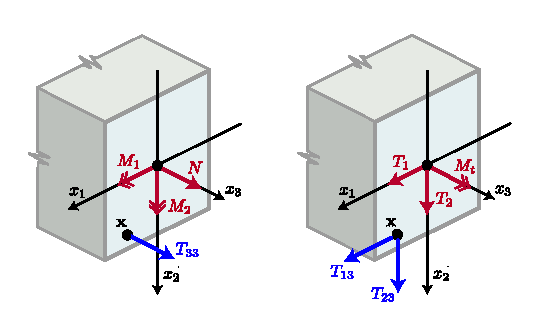
\includegraphics[scale=1.2]{figure/equilibrio/sollecitazione}
	\caption{Caratteristiche della sollecitazione.}
	\label{fig:sollecitazione}
\end{figure}



\section{Equazioni puntuali di equilibrio}
Per determinare le equazioni puntuali di equilibrio nel caso della trave conviene partire dagli assiomi di Eulero e specializzarli per la geometria in esame, che qui ripetiamo per comodità:
\begin{equation}
	\begin{aligned}\label{Eul}
	&\rb(\Pi)=\int_{\Pi}\bb+ \int_{\partial \Pi_e} \sb +\int_{\partial\Pi_i} \Tb \nb,\\
	&\mb_{\xb_0}(\Pi)=\int_{\Pi}(\xb-\xb_0)\times\bb+ \int_{\partial \Pi_e} (\xb-\xb_0)\times\sb +\int_{\partial\Pi_i} (\xb-\xb_0)\times\Tb \nb
\end{aligned}
\end{equation}
dove $\Pi\subset\Omega$. Adesso $\Omega\equiv\Tc$. Con l'idea di localizzare, scegliamo una parte di $\Tc$ che abbia essa stessa la ``forma di trave'':
\begin{equation}
\Cc_\varepsilon=\Sc\times\Ic_\varepsilon, \qquad \Ic_\varepsilon\coloneqq (z, z+\varepsilon),
\end{equation}
dove abbiamo identificato $z\equiv x_3$.
La porzione $\Cc_\varepsilon$ è spesso detta \textit{concio di trave}. La frontiera di $\Cc_\varepsilon$ è composta di due parti: il mantello $\partial \Sc \times \Ic_\varepsilon$, che corrisponde a $\partial\Pi_e$ e le due basi aventi normale $\eb_3$ e $-\eb_3$,  corrispondenti alle sezioni in $z$ e $z+\varepsilon$, che realizzano $\partial\Pi_i$ (v. Fig. \eqref{fig:concio})


\begin{figure}[h]
	\centering
	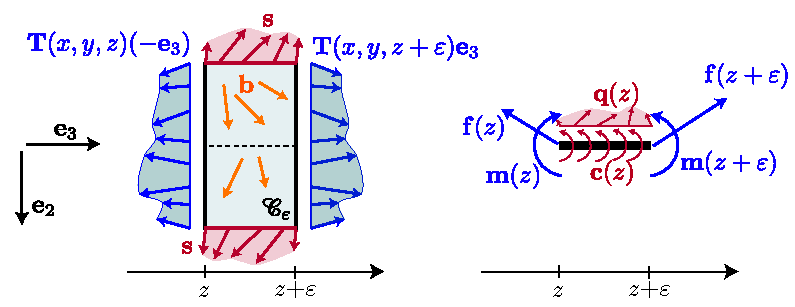
\includegraphics[width=0.9\linewidth]{figure/equilibrio/concio}
	\caption{Un concio di trave $\Cc_\varepsilon\varepsilon$ e la riduzione dei campi alla linea d'asse.}
	\label{fig:concio}
\end{figure}





Facendo uso del teorema di Fubini-Tonelli, la \eqref{Eul}$_1$ diventa allora
\begin{equation}
\rb(\Cc_\varepsilon)=\int_{\Ic_\varepsilon}\left(\int_{\Sc}\bb+\int_{\partial\Sc}\sb\right)-\int_{\Sc}\Tb(\cdot, \cdot, z)\eb_3+\Tb(\cdot, \cdot, z+\varepsilon)\eb_{3}=\mathbf{0}.
\end{equation}
Definendo
\begin{equation}\label{qb}
\qb\coloneqq\int_{\Sc}\bb+\int_{\partial\Sc}\sb
\end{equation}
il carico per unità di lunghezza della trave generato dalle forze $\bb$ e $\sb$, ricordando la \eqref{f}, la condizione di equilibrio a traslazione diventa
\begin{equation}
\int_{\Ic_\varepsilon}\qb(z)\dd z-\fb(z)+\fb(z+\varepsilon)=0.
\end{equation}
Dividiamo adesso per la misura dell'intervallo e mandiamo $\varepsilon$ a zero:
\begin{equation}
\lim_{\varepsilon\to 0}\left(\frac{1}{\varepsilon}\int_{\Ic_\varepsilon}\qb(z)\dd z +\frac{\fb(z+\varepsilon)-\fb(z)}{\varepsilon} \right)=\qb(z)+\fb'(z).
\end{equation}

L'equilibrio a traslazione di $\Cc_\varepsilon$ si tramuta dunque nell'equazione puntuale di equilibrio per la trave
\begin{definition}
	\begin{equation}\label{equil1}
\qb(z)+\fb'(z)=\mathbf{0}.
\end{equation}
\end{definition}
Rappresentando i carichi nella base $\{\eb_i\}$
\begin{equation}
\qb=p_1 \eb_1+p_2 \eb_2+ q \eb_3,
\end{equation}
la \eqref{equil1} può essere scritta per componenti come
\begin{definition}
	\begin{equation}
\begin{cases}
&p_1(z)+T_1'(z)=0,\\
&p_2(z)+T_2'(z)=0,\\
& q(z)+N'(z)=0.
\end{cases}
\end{equation}
\end{definition}

Vediamo adesso qual è la conseguenza dell'equilibrio alla rotazione \eqref{Eul}$_2$, scegliendo $\xb_0=z\,\eb_3$ e il solito concio $\Cc_\varepsilon$:
\begin{equation}\label{cb}
	\begin{aligned}
\mb_{\xb_0}(\Cc_\varepsilon)&=\int_{\Ic_\varepsilon}\left( \int_{\Sc} \pb \times \bb+\int_{\partial\Sc}\pb\times\sb\right)-\int_{\Sc}\pb\times\Tb(\cdot, \cdot, z)\eb_3\\
&+\int_{\Sc}(\pb+\varepsilon \eb_3)\times\Tb(\cdot, \cdot, z+\varepsilon)\eb_3=\mathbf{0}.
\end{aligned}
\end{equation}
Indichiamo con
\begin{equation}
	\cb\coloneqq\int_{\Sc} \pb \times \bb+\int_{\partial\Sc}\pb\times\sb
\end{equation}
le coppie per unità di lunghezza generate dal momento delle forze $\bb$ e $\sb$. Possiamo quindi scrivere
\begin{equation}
\int_{\Ic_\varepsilon} \cb(z)-\mb(z)+\mb(z+\varepsilon)+\varepsilon\eb_3\times \fb(z+\varepsilon)=\mathbf{0};
\end{equation}
dividendo per $\varepsilon$ e mandandolo a zero, si ottiene:
\begin{equation}
	\begin{aligned}
&\lim_{\varepsilon \to 0}\left(\frac{1}{\varepsilon}\int_{\Ic_\varepsilon} \cb(z)+\frac{\mb(z+\varepsilon)-\mb(z)}{\varepsilon}+\eb_3\times \fb(z+\varepsilon)\right)\\
&=\cb(z)+\mb'(z)+\eb_{3}\times\fb(z)
	\end{aligned}
\end{equation}

L'equilibrio a rotazione di $\Cc_\varepsilon$ si tramuta dunque nell'equazione puntuale di equlibrio per la trave
\begin{definition}
	\begin{equation}\label{equil2}
	\cb(z)+\mb'(z)+\eb_{3}\times\fb(z)=\mathbf{0}.
\end{equation}
\end{definition}
Rappresentando le coppie $\cb$ nella base $\{\eb_i\}$
\begin{equation}
\cb=c_1 \,\eb_1+c_2\,\eb_2+ c_t\,\eb_3,
\end{equation}
le equazioni \eqref{equil2} possono essere scritte per componenti:
\begin{definition}
	\begin{equation}
\begin{cases}
&c_1(z)+M_1'(z)-T_2(z)=0,\\
&c_2(z)+M_2'(z)+T_1(z)=0,\\
&c_t(z)+M_t'(z)=0.
\end{cases}
\end{equation}
\end{definition}

\begin{figure}[h!]
	\centering
	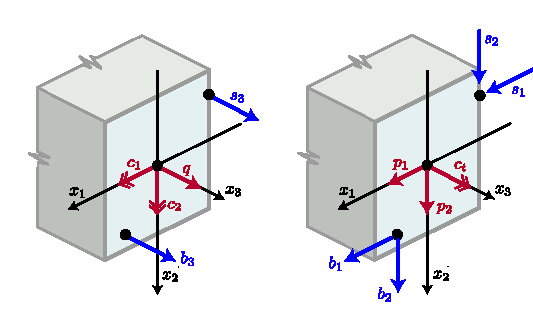
\includegraphics[scale=1.2]{figure/equilibrio/carichi}
	\caption{Carichi agenti sulla trave.}
	\label{fig:carichi}
\end{figure}



Possono darsi casi di interesse tecnico in cui i carichi esterni, ridotti alla linea d'asse, siano applicati in regioni estremamente piccole, tanto da poterli considerare delle forze concentrate. In tal caso le \eqref{equil1} e \eqref{equil2} non possono più valere, dato che i campi $\fb$ e $\mb$ non sono abbastanza regolari da poterne definire la derivata. 

Per convincersene, basta considerare una porzione di trave come quella di Fig. \ref{fig:concio}, ma soggetta a delle forze concentrate che chiamiamo $\qb_o=P_1 \eb_1+P_2\eb_2+Q \eb_3$ e $\cb_o=C_1 \eb_1+C_2 \eb_2+C_t\eb_3$.

\begin{figure}[h]
	\centering
	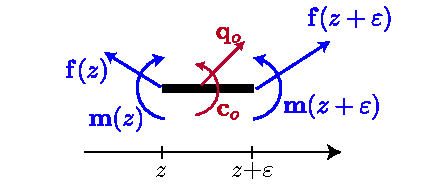
\includegraphics[width=0.45\linewidth]{figure/equilibrio/salto}
	\caption{}
	\label{fig:salto}
\end{figure}

In questo caso abbiamo
\begin{equation}
\fb(z+\varepsilon)-\fb(z)+\qb_o=\mathbf{0}, \qquad \mb(z+\varepsilon)-\mb(z)+\cb_o=\mathbf{0},
\end{equation}
ovvero, passando al limite per $\varepsilon\to 0$,
\begin{definition}
	\begin{equation}\label{disccat}
\jump{\fb}+\qb_o=\mathbf{0}, \qquad \jump{\mb}+\cb_o=\mathbf{0}
	\end{equation}
\end{definition}
dove 
\begin{equation}
\jump{\varphi}\coloneqq \varphi^+-\varphi^- 
\end{equation}
indica il \textit{salto} della funzione $\varphi$ in un punto di discontinuità. Scritte in componenti, le 
\eqref{disccat} diventano
\begin{definition}
\begin{equation}
	\begin{aligned}
&\jump{T_1}+P_1=0, \qquad &&\jump{T_2}+P_2=0, \qquad &&\jump{N}+Q=0,\\
&\jump{M_1}+C_1=0, &&\jump{M_2}+C_2=0, &&\jump{M_t}+C_t=0.\\
\end{aligned}
\end{equation}
\end{definition}






\section{La trave piana}


\begin{figure}[h]
	\centering
	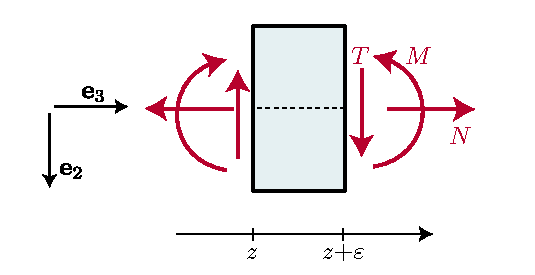
\includegraphics[width=0.5\linewidth]{figure/equilibrio/concio_piano}
	\caption{}
	\label{fig:conciopiano}
\end{figure}


\begin{definition}
	\begin{equation}\label{eqequil}
	\begin{cases}
	&p(z)+T'(z)=0,\\
	& q(z)+N'(z)=0,\\
	&c(z)+M'(z)-T(z)=0.\\
	\end{cases}
\end{equation}
\end{definition}

\begin{definition}
	\begin{equation}\label{eqequil1}
		\begin{aligned}
			&\jump{T}+P=0,  \qquad \jump{N}+Q=0,\qquad \jump{M}+C=0.
		\end{aligned}
	\end{equation}
\end{definition}

%\section{La trave di Eulero Bernoulli}
%\begin{definition}
%	\begin{equation}
%	c'(z)+M''(z)+p(z)=0
%\end{equation}
%\end{definition}

%\section{Equazione dei lavori virtuali}

\section{I vincoli}
Nella sezione \ref{vincolicin} si è data una caratterizzazione cinematica dei vincoli. Da un punto di vista dinamico, possiamo affermare che in corrispondenza di una prescrizione di natura cinematica può nascere un ente dinamico (forza o coppia), chiamata reazione vincolare, necessario a mantenere il vincolo stesso. Una forza $\bm{r}_P$ ed una coppia reattiva $\bm{c}_P$ compie lavoro nullo in corrispondenza di uno spostamento consentito dal vincolo applicato nel punto $P$. Per questo motivo le reazioni hanno la direzione del moto impedito.

Ad esempio, se un carrello impedisce lo spostamento in direzione $\nb$, potrà nascere una forza reattiva diretta come $\nb$. Lo schema in Fig. \ref{fig:reazioni} chiarisce la situazione per tutti i vincoli piani considerati. 


\begin{figure}[h]
	\centering
	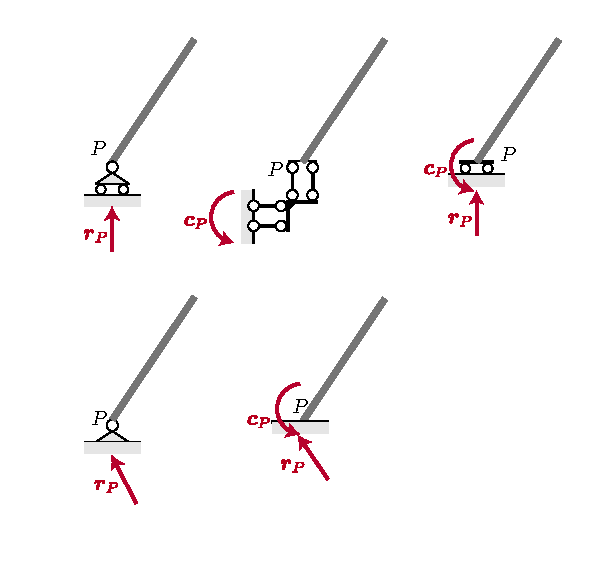
\includegraphics[width=0.7\linewidth]{figure/equilibrio/reazioni}
	\caption{}
	\label{fig:reazioni}
\end{figure}


\begin{remark}
I vincoli sono da intendersi puntuali e dunque di dimensioni nulle, benché nelle rappresentazioni grafiche sia necessario dar loro una qualche consistenza geometrica. Le reazioni vincolari pertanto vanno pensate tutte applicate nel punto $P$, anche se, per questioni grafiche può essere necessario rappresentarle diversamente. 
\end{remark}	


\section{Sistemi di travi}
Nel caso di un assemblaggio di travi tramite vincoli interni, in corrispondenza dei punti di connessione possono nascere delle reazioni vincolari, che denominiamo appunto interne. La caratterizzazione dinamica segue quella esposta per i vincoli esterni. Ovviamente, se su un corpo agisce un sistema di forze reattive, sull'adiacente ne agisce uno uguale e contrario, per il principio di azione e reazione. Tali azioni possono essere visualizzate immaginando di separare le parti in corrispondenza del vincolo, così da vedere le azioni che una parte scambia con l'altra. 

 Lo schema in Fig. \ref{fig:reazioniinterne} chiarisce la situazione per tutti il caso del carrello interno. Analoga situazione si presenta per tutti gli altri vincoli.
 
\begin{figure}[h!]
	\centering
	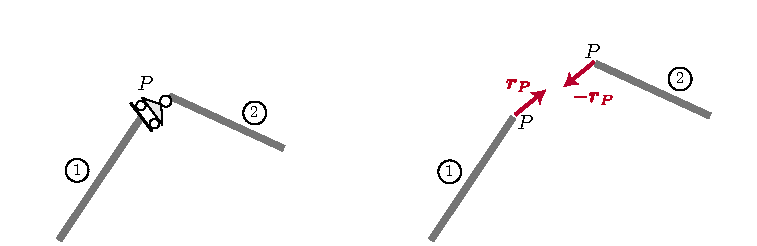
\includegraphics[width=0.8\linewidth]{figure/equilibrio/reazioni_interne}
	\caption{Reazioni interne in corrispondenza di un carrello interno.}
	\label{fig:reazioniinterne}
\end{figure}


\section{Il problema statico}
Possiamo a questo punto formulare il seguente \textit{problema statico}: 
\begin{definition}
Assegnata una certa configurazione di un sistema di travi, i carichi esterni e i vincoli, determinare  (se possibile) le reazioni vincolari in grado di bilanciare i carichi e le caratteristiche della sollecitazione.
\end{definition}

Illustriamo la modalità di soluzione tramite alcuni esempi.

Consideriamo per iniziare la trave $AB$ in figura, lunga $L$, soggetta ad una forza concentrata $\mathbf{q}_o= F(\eb_1+\eb_2)$, applicata a metà, nel punto $C$.
\begin{center}
	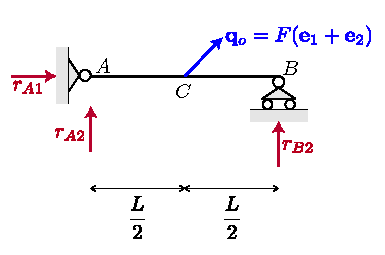
\includegraphics[width=0.5\linewidth]{figure/equilibrio/esempio1}
\end{center}

Nel punto $A$ la trave è incernierata, mentre è vincolata al terreno in $B$, tramite un carrello avente asse $\eb_2$. Pertanto, nel punto $A$ ci aspettiamo che possa nascere una forza reattiva di inclinazione qualunque ${\bm r}_A=r_{A1}\eb_1+r_{A2}\eb_2$; nel punto $B$ invece può nascere solo una reazione diretta come l'asse del carrello ${\bm r}_{B}=r_{B2}\eb_2$.

Affinché la trave sia in equilibrio, è necessario che siano soddisfatti gli assiomi di Eulero, ovvero che siano nulli il risultante e il momento risultante rispetto ad un qualunque polo del sistema di forze agenti sul corpo. Ovvero, scegliendo come polo dei momenti A
\begin{equation}
\rb ={\bm r}_A+{\bm r}_B+\qb_o=\mathbf{0}, \qquad \mb_A=\overrightarrow{AC}\times \qb_o+\overrightarrow{AB}\times{\bm r}_B=\mathbf{0}.
\end{equation}
Scrivendo le due condizioni per componenti, ci troviamo a dover risolvere il sistema
\begin{equation}
\begin{cases}
r_{A1}+F=0,\\
r_{A2}+r_{B2}+F=0\\
\dfrac{FL}{2}+r_{B2}L=0,
\end{cases}
\end{equation}
la cui soluzione è immediato determinare:
\begin{equation}
r_{A1}=-F, \qquad r_{A2}=-\frac{F}{2}, \qquad r_{B2}=-\frac{F}{2}.
\end{equation}
Riportiamo sotto i risultati determinati, rappresentando il cosiddetto \textit{schema di corpo libero}, ovvero uno schema in cui sia presente il corpo privo di vincoli (libero) con tutte le forze su di esso agenti, siano attive che reattive.

\begin{center}
	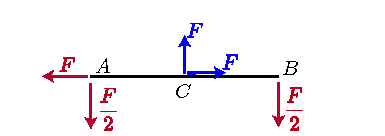
\includegraphics[width=0.5\linewidth]{figure/equilibrio/esempio1_2}
\end{center}

Possiamo adesso passare alla determinazione delle caratteristiche della sollecitazione. Per farlo, possiamo agire in due modi:
\begin{itemize}
	\item Integrando le equazioni puntuali di equilibrio \eqref{eqequil} e \eqref{eqequil1};
	\item Utilizzando la definizione di caratteristiche della sollecitazione e gli assiomi di Eulero formulati su una parte, piuttosto che su tutta la trave.
\end{itemize}

La presenza di forze concentrate nel punto $C$ ci porta a concludere che $N$ e $T$ non sono continui. Inoltre, alla luce di \eqref{eqequil}$_3$, neppure $M'$ sarà continua, benché invece lo sia $M$, visto che non sono presenti coppie concentrate. Dobbiamo dunque determinare i seguenti campi:



\begin{equation}
	\begin{aligned}
		N(z) &= \begin{cases}
			\begin{aligned}
				&N_1(z) \quad &&0<z<L/2 \\
				&N_2(z) \quad &&L/2<z<L
			\end{aligned}
		\end{cases}, \quad 
		T(z) = \begin{cases}
			\begin{aligned}
				&T_1(z) \quad &&0<z<L/2 \\
				&T_2(z) \quad &&L/2<z<L
			\end{aligned}
		\end{cases}, \\
		M(z) &= \begin{cases}
			\begin{aligned}
				&M_1(z) \quad &&0<z<L/2 \\
				&M_2(z) \quad &&L/2<z<L
			\end{aligned}
		\end{cases}.
	\end{aligned}
\end{equation}

Procediamo con il primo metodo. Integrando le \eqref{eqequil} si ottiene
\begin{equation}
	\begin{aligned}
&N_1(z)=a_1, \quad N_2(z)=a_2,\\ 
&T_1(z)=b_1, \quad T_2(z)=b_2, \\ 
& M_1(z)=b_1(z)+c_1, \quad  M_2(z)=b_2(z)+c_2,
	\end{aligned}
\end{equation}
dove le costanti di integrazione $a_1$, $a_2$, $b_1$, $b_2$, $c_1$ e $c_2$ possono essere facilmente  determinate una volta che si siano trovate le reazioni vincolari nei punti $A$ e $B$. Infatti, dallo schema di corpo libero, adoperando la convenzione sui segni dettata dalla Fig. \ref{fig:conciopiano}, possiamo concludere che
\begin{equation}
	N_1(0)=F, \quad N_2(L)=0, \quad T_1(0)=-\frac F2,  \quad T_2(L)=\frac F2, \quad M_1(0)=M_2(L)=0.
\end{equation}
Tanto basta per concludere che
\begin{equation}
a_1=F, \quad a_2=0, \quad b_1=-\frac F2, \quad  b_2=\frac F2, \quad c_1=0, \quad c_2=-\frac{FL}{2}
\end{equation}
e dunque

\begin{equation}
	\begin{aligned}
		N(z) &= \begin{cases}
			\begin{aligned}
				&F \quad &&0<z<L/2 \\
				&0\quad &&L/2<z<L
			\end{aligned}
		\end{cases}, \quad 
		T(z) = \begin{cases}
			\begin{aligned}
				&-\frac{F }{2}\quad &&0<z<L/2 \\
				&\frac{F }{2}\quad &&L/2<z<L
			\end{aligned}
		\end{cases}, \\
		M(z) &= \begin{cases}
			\begin{aligned}
				&-\frac{F }{2}z \quad &&0<z<L/2 \\[.3cm]
				&\frac{F }{2}\left(z-L\right)\quad &&L/2<z<L.
			\end{aligned}
		\end{cases}.
	\end{aligned}
\end{equation}

Osserviamo che le \eqref{eqequil1} risultano soddisfatte; infatti, nel punto $C$
\begin{equation}
\jump{N}=N^+-N^-=-F, \qquad \jump{T}=T^+-T^-=F, \qquad \qquad \jump{T}=0.
\end{equation}

Delle funzioni appena determinate si può dare una rappresentazione grafica efficace a comprenderne in maniera rapida l'andamento e per individuare i punti maggiormente sollecitati, nota come diagrammi delle caratteristiche della sollecitazione.

\begin{center}
		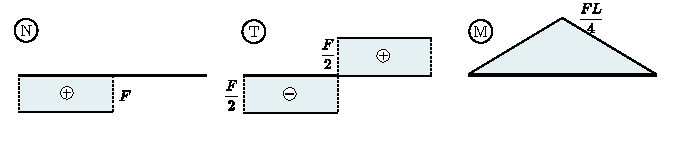
\includegraphics[width=1\linewidth]{figure/equilibrio/esempio1_3}
\end{center}

È consuetudine indicare nel diagramma dello sforzo normale e del taglio il segno. Per quanto riguarda il diagramma del momento, si conviene di disegnarlo dalla parte delle fibre tese. 

Vediamo adesso come determinare le caratteristiche della sollecitazione senza integrare le \eqref{eqequil1}, utilizzando la definizione di caratteristiche della sollecitazione e gli assiomi di Eulero formulati su una parte, piuttosto che su tutta la trave. A tale scopo isoliamo una parte di trave, compresa tra $A$ ed un punto generico a distanza $z$ da $A$. La situazione è schematizzata sotto.

\begin{center}
	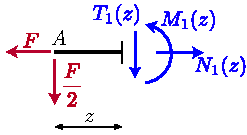
\includegraphics[width=.3\linewidth]{figure/equilibrio/esempio1_4}
\end{center}

La parte isolata, per gli assiomi di Eulero, dev'essere bilanciata. Basta allora imporre l'equilibrio a traslazione e rotazione della parte isolata per concludere che
\begin{equation}
N_1(z)=F, \qquad T_1(z)=-\frac{F}{2}, \qquad M_1(z)=-\frac{F}{2}z.
\end{equation}

Immaginando di isolare una parte tra $C$ e $B$ come sotto si determinano le altre funzioni:

\begin{center}
	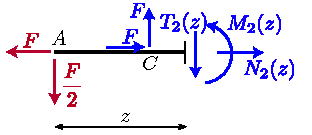
\includegraphics[width=.35\linewidth]{figure/equilibrio/esempio1_5}
\end{center}

\begin{equation}
	N_2(z)=0, \qquad T_2(z)=\frac{F}{2}, \qquad M_2(z)=\frac{F}{2}(z-L).
\end{equation}


\subsubsection{Il tracciamento qualitativo delle caratteristiche della sollecitazione}
Ai fini della determinazione delle caratteristiche della sollecitazione, a partire  dall'assegnazione dei carichi esterni dalle densità di forze e coppie assegnate, vale la pena sottolineare alcuni aspetti utili per tracciarne l'andamento in modo \emph{qualitativo}, cioè senza la necessità di specificare le funzioni che ne descrivono i campi:
\begin{itemize}[]
	\item[{ a})] dalle equazioni  puntuali di equilibrio \eqref{eqequil} si evince che:
	\begin{itemize}
		\item per tratti di trave che non siano soggetti a  \emph{carichi}  i diagrammi dello sforzo normale e del taglio sono \emph{uniformi}, il diagramma del momento flettente è \emph{lineare}. 
		Per tracciare l'andamento di $N\,$ e $T\;$ sul tratto è sufficiente conoscere il valore in uno dei due estremi; per tracciare l'andamento di $M\;$ è sufficiente conoscere il valore assunto nei due estremi e collegarli con un tratto di retta.
		\item per tratti di trave che siano soggetti  di carichi uniformi, i diagrammi dello sforzo normale e del taglio sono \emph{lineari}, il diagramma del momento flettente è \emph{parabolico}.
		Per tracciare l'andamento di $N\;$ e $T\;$ sul tratto è sufficiente conoscere il valore assunto nei due estremi e collegarli con un tratto di retta.
		Per tracciare qualitativamente l'andamento di $M\;$  si può utilizzare il valore e la tangente nei due estremi, verificando se ci sono punti di massimo o minimo, quelli in cui $T=0$.
		\item in assenza di coppie distribuite,  la derivata del momento flettente, $M$, è pari alla forza di taglio, $T$, mentre  la derivata seconda è pari all'opposto del carico trasversale, $p$,\\
		\[M'=T,\qquad M''=-p.\] 
		Stanti queste eguaglianze differenziali si ha che in corrispondenza dei punti di nullo della forza di  taglio, il  momento flettente  attinge a un valore stazionario: di minimo quando $-p>0$, di massimo quando $-p<0$;  presenta, invece, un  flesso quando $-p=0\;$ ovvero  nei punti dove $T\;$ attinge a un valore stazionario.
		 È inoltre utile la cosiddetta \textit{analogia della fune},  basata sulla similitudine tra le equazioni che descrivono la forma di una fune tesa appesa sotto carico e quelle che descrivono il momento flettente in una trave soggetta a carichi. La forma della fune sotto carico rappresenta visivamente l'andamento del momento flettente lungo una trave soggetta a carichi distribuiti uniformemente. Pertanto se il carico è verso il basso, la concavità sarà verso l'alto, e viceversa. 
	\end{itemize}
	\item[{ b})] dalle condizioni di salto \eqref{eqequil1}
		risulta inoltre che: 
	\begin{itemize}
		\item in corrispondenza di un punto in cui è applicata una forza longitudinale $Q$ lo sforzo normale subisce un salto di $-Q$, mentre il taglio e  il momento sono continui;
		\item in corrispondenza di un punto in cui è applicata una forza trasversale $P$ la forza di taglio subisce un salto di $-P$, mentre lo sforzo normale e il momento sono continui. In assenza di coppie diffuse $c$, poiché $\jump{T}=\jump{M'}$, la tangente al diagramma del momento non sarà continua e si osserverà un punto angoloso. Anche in questo caso può tornare utile l'analogia della fune, per capire la natura del punto angoloso.
		\item in corrispondenza di un punto  in cui è applicata una coppia $C$ il momento flettente subisce un salto di $-C$,  mentre la forza di taglio e lo sforzo normale  sono continui;
		\item in presenza di una forza con entrambe  le componenti, longitudinale e trasversale, e di una coppia tutte le caratteristiche della sollecitazione subiscono un salto.
	\end{itemize}
\end{itemize}

\begin{exercise}
Si consideri la mensola in figura, soggetta ad un carico trasversale distribuito $p$. Determinare le reazioni vincolari e disegnare i diagrammi delle caratteristiche della sollecitazione.
\begin{center}
	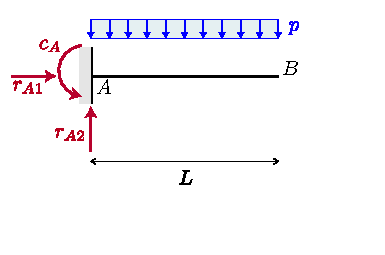
\includegraphics[width=0.45\linewidth]{figure/equilibrio/esempio2}
\end{center}
\begin{svolgimento}
Le equazioni di equilibrio globale prescrivono che
\begin{equation}
\begin{cases}
r_{A1}=0,\\
r_{A2}-pL=0,\\
m_A=c_A-\frac{pL^2}{2}=0,
\end{cases}
\end{equation}
la cui soluzione è immediata e riportata nello schema di corpo libero sotto.
\begin{center}
	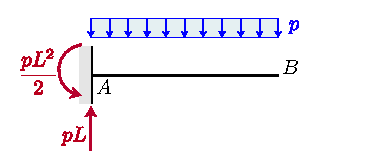
\includegraphics[width=0.45\linewidth]{figure/equilibrio/esempio2_1}
\end{center}
Non essendoci carichi orizzontali, $N=0$. La presenza di un carico distribuito trasversale costante implica che il taglio è lineare e il momento flettente parabolico.
Per disegnare il taglio, è sufficiente conoscerne i due valori agli estremi: in $A$ vale $pL$, mentre è nullo in $B$. Per disegnare il momento flettente, consideriamo i valori agli estremi: $pL^2/2$ in $A$ e nullo in $B$;  osserviamo inoltre che $T=0$ nel punto $B$, che significa che in quel punto il momento ha un punto stazionario e quindi la pendenza della retta tangente al grafico di $M$ è nulla; infine, sfruttando l'analogia della fune, intuiamo che la concavità è verso l'alto.
\begin{center}
	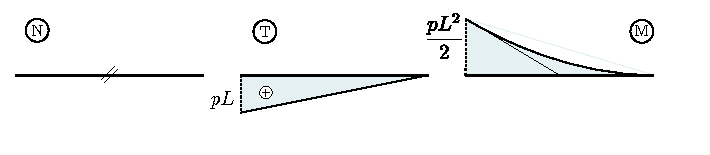
\includegraphics[width=.8\linewidth]{figure/equilibrio/esempio2_2}
\end{center}
\end{svolgimento}

\end{exercise}
\subsection{Sistemi di travi}\label{sisstr}
Si consideri il sistema di due travi in figura, incernierato a terra in $A$ e $B$ e collegate tra loro in $C$ tramite un'altra cerniera. Il sistema strutturale è piuttosto ricorrente ed è detto \textit{arco a tre cerniere}.

\begin{center}
	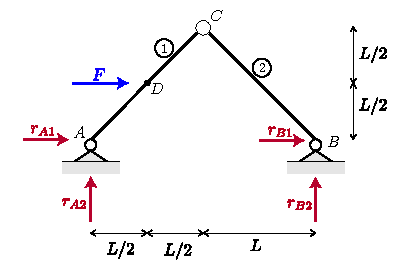
\includegraphics[scale=1.2]{figure/equilibrio/esempio3}
\end{center}

Trovandoci di fronte ad un sistema di due travi, occorre rendersi conto che l'equilibrio globale non è sufficiente a garantirne l'equilibrio. È infatti necessario che gli assiomi di Eulero valgano \textit{per ogni} parte. In maniera più precisa, la presenza un vincolo interno consente, in linea di principio, un movimento relativo tra le parti. La cerniera in $C$ consente alla trave $AC$ di ruotare attorno a $C$ rispetto alla trave $AB$. Per impedire questa evenienza e garantire l'equilibrio del sistema è dunque necessario richiedere che sia soddisfatto l'equilibrio a rotazione attorno a $C$ di una delle due parti, ad esempio la 2:
\begin{equation}
0=m_C^{(2)}=r_{B1}L+r_{B1}L.
\end{equation}
Oltre alla condizione di \textit{equilibrio parziale}, occorre comunque garantire le condizioni di \textit{equilibrio globale}:
\begin{equation}
\rb=\mathbf{0}, \qquad \mb_A=\mathbf{0},
\end{equation}
avendo scelto $A$ come polo dei momenti. Ne segue che otteniamo il seguente sistema per le incognite $r_{A1}$, $r_{A2}$, $r_{B1}$, $r_{B2}$:
\begin{equation}\label{sys}
\begin{cases}
r_{A1}+r_{B1}+F=0,\\[.2cm]
r_{A2}+r_{B2}=0,\\[.2cm]
2 r_{B2}L-\dfrac{FL}{2}=0,\\[.2cm]
r_{B1}L+r_{B2}L=0,
\end{cases}
\end{equation}
la cui soluzione è
\begin{equation}
r_{A1}=-\frac{3}{4}F, \qquad r_{A2}=-\frac F4, \qquad r_{B1}=-\frac F4, \qquad r_{B2}=\frac F4.
\end{equation}

Per determinare le reazioni dei vincoli interni, occorre passare per gli schemi di corpo libero per ogni corpo; in corrispondenza del vincolo, occorre mettere il sistema di reazioni che esso può esplicare, come in figura.
\begin{center}
	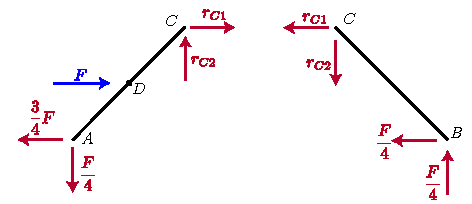
\includegraphics[scale=1.2]{figure/equilibrio/esempio3_1}
\end{center}
 Per determinare le forze reattive $r_{C1}$ e $r_{C2}$ basta allora richiedere che sia garantito l'equilibrio a traslazione orizzontale e verticale di una delle due travi, trovando
 \begin{equation}
 	r_{C1}=-\frac F4, \qquad r_{C2}=\frac{F}{4}.
 \end{equation}
 
 \begin{exercise}
 Si consideri il sistema di travi in figura. Determinare le reazioni vincolari.
 
 \begin{center}
 	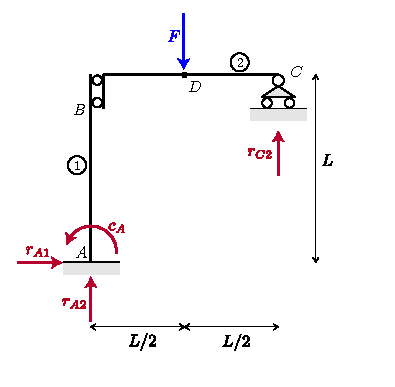
\includegraphics[scale=1.2]{figure/equilibrio/esempio4}
 \end{center}
 
 \begin{svolgimento}
 La presenza del glifo in $B$ richiede che il movimento consentito da quel vincolo sia impedito. Visto che il glifo consente la traslazione verticale relativa, scriviamo pertanto la condizione di equilibrio parziale, riferita ad una delle due parti. Scegliendo la parte 2:
 \begin{equation}
 r_{C2}=F.
 \end{equation}
 Possiamo adesso procedere con gli equilibri globali:
 \begin{equation}
 \begin{cases}
 	r_{A1}=0,\\[.2cm]
 	r_{A2}+r_{C2}-F=0,\\[.2cm]
 	m_A=r_{C2}L-\dfrac{F}{L}+c_A=0.
 \end{cases}
 \end{equation}
 La soluzione è immediata:
 \begin{equation}
r_{A2}=0, \qquad  r_{C2}=F, \qquad c_A=-\frac F2.
 \end{equation}
 Procediamo adesso con la determinazione delle reazioni interne, usando gli schemi di corpo libero.
  \begin{center}
 	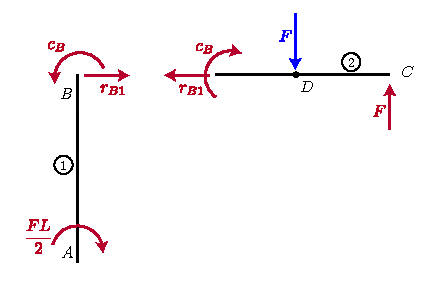
\includegraphics[scale=1.2]{figure/equilibrio/esempio4_1}
 \end{center}
 L'equilibrio a traslazione orizzontale della parte 1 impone che
 \begin{equation}
 	r_{B1}=0.
 \end{equation}
 L'equilibrio a rotazione attorno a $B$ della parte 1 implica 
 \begin{equation}
 m_B^{(1)}=c_B-\frac{FL}{2}=0 \qquad \Longrightarrow\qquad c_B=\frac{FL}{2}.
 \end{equation}
 \end{svolgimento}
 
 \end{exercise}

\begin{exercise}
Si consideri la trave in figura. Tracciare qualitativamente i diagrammi delle caratteristiche della sollecitazione.
\begin{center}
	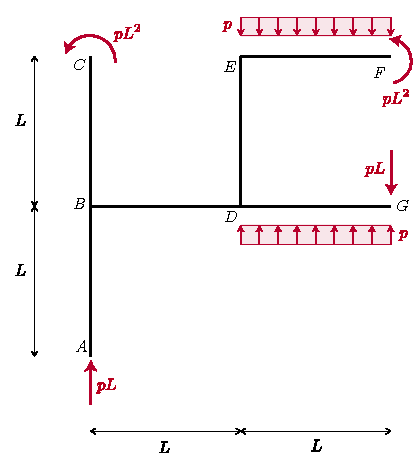
\includegraphics[scale=1.2]{figure/equilibrio/esempio5}
\end{center}

\begin{svolgimento}
Iniziamo dallo sforzo normale. Essendo $q=0$ su tutta la trave, $N$ sarà costante a tratti. La determinazione della costante è immediata per quei tratti che contemplano un estremo libero: in per $AB$ vediamo che $N=-pL$ in A; per $BC$ vediamo che $N=0$; per $EF$ $N=0$ in $F$; per $DG$ $N=0$ in $G$. Mancano da determinare gli sforzi normali dei tratti interni, ovvero $BD$ e $ED$. Per farlo basta effettuare un taglio di Eulero in un qualunque punto di $BD$ e $ED$, isolare una parte e richiedere che sia in equilibrio nella direzione di $N$. Ci si accorge quindi subito che $N=0$ in $BD$ e $N=-pL$ in $ED$. Il diagramma è rappresentato sotto.

\begin{center}
	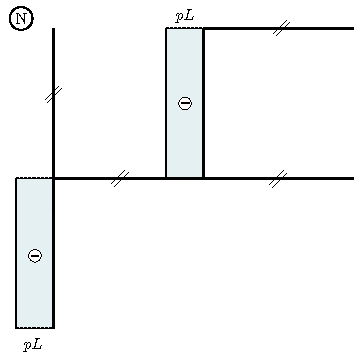
\includegraphics[scale=1.2]{figure/equilibrio/esempio5_1}
\end{center}

Passiamo allo sforzo di taglio. Essendoci su $EF$ e $DG$ un carico distribuito costante, sappiamo che lì il taglio sarà lineare, mentre altrove costante. Ragionando come per lo sforzo normale, è immediato vedere che $T=0$ in $AC$, $T=pL$ su $BD$ e $T=0$ su $ED$. Per quanto riguarda il tratto $EF$, essendo lì il taglio lineare, è necessario determinarne il valore nei punti estremi; per quanto riguarda il punto $F$, essendo un punto esterno, si vede che $T=0$; per determinare il valore del taglio in $E$ serve effettuare un taglio di Eulero in quel punto, isolando ad esempio la parte $EF$ e richiedendo che sia soddisfatto l'equilibrio nella direzione del taglio, il che porta a concludere che $T_E=pL$. analogamente ragioniamo per l'altro tratto in cui il taglio è lineare, $DG$: in $G$ il taglio vale $pL$; effettuando un taglio di Eulero in $D$ e isolando $DG$ si vede subito che il taglio è nullo. Il diagramma è rappresentato sotto.

\begin{center}
	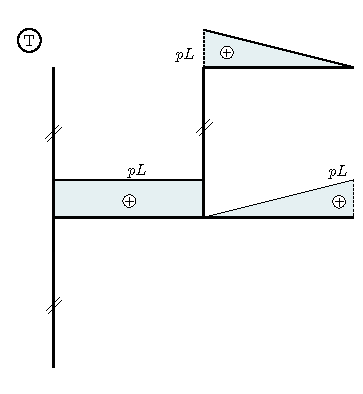
\includegraphics[scale=1.2]{figure/equilibrio/esempio5_2}
\end{center}

Concludiamo con il diagramma del momento flettente. Visto che $M'=T$, dove  $T$ è nullo, $M$ sarà costante, dove $T$ è costante $M$ sarà lineare e dove $T$ è lineare $M$ sarà parabolico.
Nel tratto $AB$ il momento è dunque costante ed è $M=0$, visto che nel punto estremo $A$ non vi sono coppie. In $BC$ è ancora costante e vale quanto la coppia applicata in $C$, che tende le fibre di destra. Sul tratto $BD$ è lineare, occorre dunque determinare i valori in $B$ e $D$ con i soliti tagli di Eulero. In $ED$ il momento è costante e dunque basta effettuare un taglio di Eulero in un punto qualunque. Su $EF$ dovremo disegnare una parabola: i valori estremi si determinano guardando il punto esterno $F$, dove c'è una coppia $pL^2$ che tende le fibre di sotto, ed effettuando un taglio di Eulero in $E$ e guardando a destra; essendo il carico distribuito verso il basso, la concavità sarà verso l'alto, per l'analogia della fune; infine, poiché il taglio in $F$ è nullo, in quel punto la pendenza della retta tangente a $M$ sarà nulla.  In maniera simile si ragiona per $DG$: dopo aver determinato i valori agli estremi, si osserva che la concavità sarà verso il basso e che in $D$ la pendenza della tangente a $M$ sarà nulla. Il diagramma è rappresentato sotto.
\begin{center}
	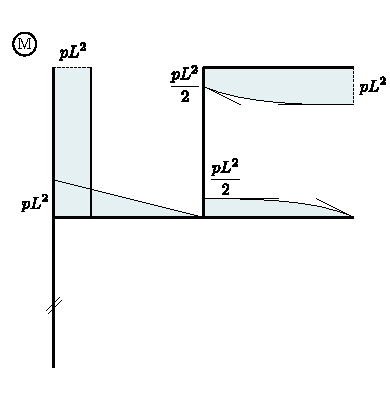
\includegraphics[scale=1.2]{figure/equilibrio/esempio5_3}
\end{center}
\end{svolgimento}
\end{exercise}


\subsection{Classificazione strutturale}\label{classif}
Il problema della determinazione delle reazioni vincolali può essere formalmente scritto in forma matriciale come
\begin{equation}\label{Arf}
[\Ab][\bm{r}]+[\fb]=[\mathbf{0}],
\end{equation}
dove $[\bm{r}]$ è il vettore colonna che contiene il numero di incognite date dalle reazioni vincolari, $[\fb]$ il vettore delle forze e  $[\Ab]$ la cosiddetta \textit{matrice di equilibrio}. Esistenza e unicità della soluzione del problema lineare \eqref{Arf} sono regolati dai ben noti teoremi dell'algebra lineare, in particolare dal teorema di Rouché-Capelli.

Ad esempio, con riferimento al sistema \eqref{sys} relativo all'esempio illustrato nella Sez. \ref{sisstr}, avremmo
%
%\begin{equation}\label{sys}
%	\begin{cases}
%		r_{A1}+r_{B1}+F=0,\\[.2cm]
%		r_{A2}+r_{B2}=0,\\[.2cm]
%		2 r_{B2}L-\dfrac{FL}{2}=0,\\[.2cm]
%		r_{B1}L+r_{B1}L=0,
%	\end{cases}
%\end{equation}
%avremmo
\begin{equation}
	\begin{bmatrix}
		1 & 1 & 0 & 0  \\
		0 & 0 & 1 & 1  \\
		0 & 0 & 0 & 2L  \\
		0 & L & 0 & L 
	\end{bmatrix}
	\begin{bmatrix}
		r_{A1} \\
		r_{B1} \\
		r_{A2} \\
		r_{B2} 
	\end{bmatrix}+
	\begin{bmatrix}
		F\\
		0 \\
	-\frac{FL}{2} \\
	0
	\end{bmatrix}
	=
	\begin{bmatrix}
		0 \\
		0 \\
		0 \\
		0
	\end{bmatrix}
\end{equation}
e dunque
\begin{equation}
	[\Ab]=\begin{bmatrix}
		1 & 1 & 0 & 0  \\
		0 & 0 & 1 & 1  \\
		0 & 0 & 0 & 2L  \\
		0 & L & 0 & L 
	\end{bmatrix}, \qquad
	[{\bm r}]=\begin{bmatrix}
		r_{A1} \\
		r_{B1} \\
		r_{A2} \\
		r_{B2} 
	\end{bmatrix}, \qquad 
	[\fb]=\begin{bmatrix}
	F\\
	0 \\
	-\frac{FL}{2} \\
	0
	\end{bmatrix}.
\end{equation}
Non è difficile verificare che la matrice $	[\Ab]$ è di rango massimo e che questo coincide col rango della matrice orlata, portando a concludere che la soluzione esiste ed è unica, come d'altra parta abbiamo constatato risolvendo il sistema.

In generale, la matrice del sistema da risolvere ha un numero di incognite  pari alla molteplicità totale dei vincoli presenti nel sistema, che indichiamo con $\mathscr{v}$, mentre il numero di equazioni è pari a $3\times$(numero dei corpi)$=\mathscr{g}$, i gradi di libertà del sistema. La matrice $	[\Ab]$ ha dunque $\mathscr{g}$ righe e $\mathscr{v}$ colonne e dunque può essere rivista come un operatore lineare $[\Ab ]\,:\, \Ro^\mathscr{v} \to \Ro ^\mathscr{g}$.

Piuttosto che studiare le proprietà algebriche di $	[\Ab]$, cerchiamo un modo spedito per comprendere se la soluzione del problema esiste e se è unica, sfruttando alcune proprietà generali, con l'obiettivo di classificare i sistemi di travi.

Ricordiamo innanzitutto la definizione di nucleo e immagine di $\Ab$:
\begin{equation}
\operatorname{Ker}[\Ab]=\{\textrm{spazio nullo di $[\Ab]$}\}=\{ [{\bm r}]\in \Ro^\mathscr{v}\,:\, [\Ab][{\bm r}]=[\mathbf{0}] \},\
\end{equation}
\begin{equation}
\operatorname{Im}[\Ab]=\{\textrm{spazio generato dalle colonne di $[\Ab]$}\}=\{ [\ub] \in \Ro ^{\mathscr{g}}\,:\, [\ub]= [\Ab][{\bm r}]\}
\end{equation}

Date queste definizioni, i vettori appartenenti a $\operatorname{Ker}[\Ab]$ rappresentano le \textit{reazioni vincolari autoequilibrate}, ovvero quelle reazioni  provocate da vincoli sovrabbondanti. Ad esempio, nella trave seguente
\begin{center}
	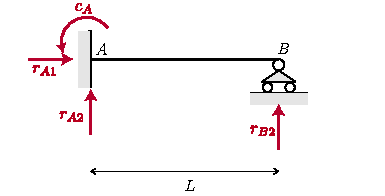
\includegraphics[scale=1.2]{figure/equilibrio/iperstatica}
\end{center}
possiamo scrivere le equazioni di equilibrio
\begin{equation}
\begin{cases}
r_{A1}=0,\\
r_{A2}+r_{B2}=0,\\
c_A+r_{B2}L=0,
\end{cases}
\end{equation}
la cui soluzione corrisponde un sistema di forze \textit{autoequilibrato} 
\begin{equation}
r_{A1}=0, \qquad r_{A2}=-r_{B2}, \qquad c_A=-r_{B2}L.
\end{equation}
La soluzione dipende da un parametro, che in questo caso abbiamo scelto come $r_{B2}$. Un sistema di questo tipo ha un vincolo sovrabbondante e per questa ragione è detto essere una volta  \textit{iperstatico}.

La dimensione del nucleo di $[\Ab]$ individua appunto il numero dei parametri necessari a rappresentare la soluzione del problema di equilibrio corrispondente a carichi nulli ed è dunque detto \textit{grado di iperstaticità} $\mathscr{i}$:
\begin{equation}\label{ip}
\mathscr{i}\coloneqq \operatorname{dim}(\operatorname{Ker}[\Ab]).
\end{equation}


I  vettori appartenenti a $\operatorname{Im}[\Ab]$ sono quelli per cui è possibile trovare una soluzione alle equazioni di equilibrio e dunque rappresentano i \textit{carichi compatibili}. La dimensione dell'immagine di $[\Ab]$ ne definisce il rango ed è dunque pari al numero di colonne linearmente indipendenti, ovvero caratterizza il numero di vincoli che effettivamente contribuiscono all'equilibrio.  I gradi di libertà residui, dati dai gradi di libertà teorici, ovvero $\mathscr{g}$, meno quelli che sono eliminati dai vincoli effettivi definiscono la \textit{labilità} $\mathscr{l}$ del sistema:
\begin{equation}\label{ell}
\mathscr{l}\coloneqq \mathscr{g }-\operatorname{dim}(\operatorname{Im}[\Ab]).
\end{equation}




 Dal teorema di nullità più rango\footnote{Ricordiamo che il teorema di nullità più rango, detto anche teorema del rango, o teorema della dimensione, afferma che la somma tra la dimensione dell'immagine e la dimensione del nucleo di una trasformazione lineare è uguale alla dimensione del dominio di tale trasformazione lineare; equivalentemente, la somma del rango e della nullità di una matrice è uguale al numero di colonne della matrice.}, abbiamo allora che 
\begin{equation}
\operatorname{dim}(\operatorname{Ker}[\Ab])+\operatorname{dim}(\operatorname{Im}[\Ab])=\mathscr{v},
\end{equation}
che, viste le  \eqref{ip} e \eqref{ell} può essere riscritta come
\begin{definition}
	\begin{equation}\label{gmv}
\mathscr{g}-\mathscr{v}=\mathscr{l}-\mathscr{i}.
\end{equation}
\end{definition}

La formula \eqref{gmv} mostra che la differenza tra il numero di righe $\mathscr{g}$ e il numero di colonne $\mathscr{v}$ della matrice $[\Ab]$ fornisce un'informazione tra il grado di labilità e il grado di iperstaticità. 

Il sistema di travi   allora si può classificare come segue:
\begin{definition}
	\begin{itemize}
	\noindent\item \textit{Isostatico}, se $\mathscr{g}=\mathscr{v}$ e $\mathscr{l}=\mathscr{i}=0$, ovvero ci sono un numero di vincoli non sovrabbondanti ed efficacemente disposti. La soluzione del problema statico è unica.
	\item \textit{Iperstatico}, se $\mathscr{l}=0$ e $\mathscr{i}>0$, ovvero se ci sono più vincoli del necessario. Esistono $\infty^i$ soluzioni del problema statico.
	\item \textit{Labile}, se $\mathscr{l}>0$ e $\mathscr{i}=0$, ovvero se  $\mathscr{g}>\operatorname{dim}(\operatorname{Im}[\Ab])$ e dunque, nonostante la presenza di vincoli, ci sono gradi di libertà residui. La struttura è dunque capace di effettuare (piccoli) spostamenti, ovvero ammette dei \textit{cinematismi}. In generale,  la soluzione del problema statico non esiste, a meno che i carichi non siano in grado di attivare i cinematismi.
	\item \textit{Degenere}, se $\mathscr{l}=\mathscr{i}>0$. In questo caso ci sono vincoli sovrabbondanti, ma mal posti e dunque sono comunque possibili (piccoli) spostamenti.  In generale la soluzione del problema statico non esiste, a meno che i carichi non siano in grado di attivare i cinematismi.
\end{itemize}
\end{definition}

Da un punto di vista operativo, è spesso semplice determinare se $\mathscr{l}>0$, cioè se sono possibili piccoli spostamenti, utilizzando i teoremi di Aronhold--Kennedy (v. Sez \ref{sistr}). In particolare, se si determinano in maniera univoca i centri di rotazione, allora $\mathscr{l}=1$. Se invece i centri esistono,  ma non si riescono a determinare in maniera univoca $\mathscr{l}>1$. In questo caso si può introdurre un vincolo di molteplicità 1 e provare a cercare i centri; se si riescono a determinare, allora $\mathscr{l}=1+1$ e così via, se invece la determinazione non è possibile.


Facciamo degli esempi. Consideriamo il sistema in figura.
\begin{center}
	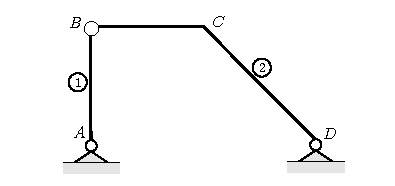
\includegraphics[scale=1.3]{figure/equilibrio/classificazione_iso}
\end{center}
Il sistema è composto da due travi e dunque ha $\mathscr{g}=2\times 3=6$ gradi di libertà. La molteplicità di ogni cerniera è pari a 2, quindi $\mathscr{v}=2+2+2=6$. Dunque $\mathscr{g}-\mathscr{v}=0$, ovvero $\mathscr{l}-\mathscr{i}=0$; ne segue che il sistema o è isostatico o è degenere. Cerchiamo di valutare dunque il grado di labilità, analizzando i possibili centri di rotazione. Se esistesse, il centro di rotazione del corpo 1 sarebbe sulla cerniera in $A$, così come quello del corpo 2 sarebbe sulla cerniera in $D$; il centro relativo tra i due sarebbe in $B$, ma la situazione è incompatibile con il primo teorema di Aronhold--Kennedy: i centri di rotazione non esistono, $\mathscr{l}=0$ e quindi il sistema è isostatico.

Consideriamo adesso il sistema in figura, composto sempre da due travi e dunque con $\mathscr{g}=2\times 3=6$ gradi di libertà.
\begin{center}
	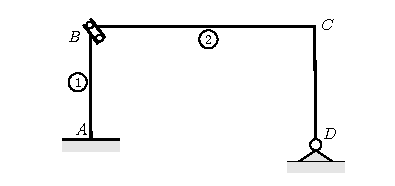
\includegraphics[scale=1.3]{figure/equilibrio/classificazione_iper}
\end{center}
La molteplicità totale dei vincoli è in questo caso $\mathscr{v}=3+2+2=7$ e allora $\mathscr{g}-\mathscr{v}=-1=\mathscr{l}-\mathscr{i}$. Dunque il sistema o è iperstatico o degenere. Vediamo se è ammesso un cinematismo,  analizzando i possibili centri di rotazione. Osserviamo che la trave 1 è incastrata in $A$ e dunque certamente non può ammettere alcun cinematismo; il punto $B$ allora è certamente fisso. Il corpo 2 allora è vincolato a terra tramite la cerniera in $D$ e tramite il glifo in $B$, dato che quel punto non può spostarsi. Il vincolo in $D$ vorrebbe che il centro di rotazione si trovasse lì, mentre il glifo in $D$ darebbe un centro di rotazione all'infinito, nella direzione dell'asse. Essendo le due circostanze incompatibili, concludiamo che il centro del secondo corpo non esiste. Allora $\mathscr{l}=0$ e $\mathscr{i}=1$, ovvero c'è un vincolo sovrabbondante, che rende il sistema iperstatico. 

Consideriamo adesso il sistema in figura.
\begin{center}
	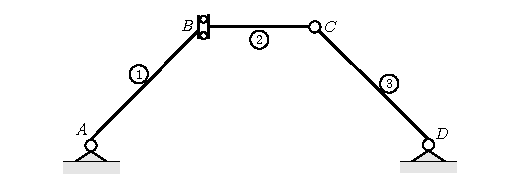
\includegraphics[scale=1.3]{figure/equilibrio/classificazione_lab}
\end{center}
Il sistema è composto  da 3 travi e dunque con $\mathscr{g}=3\times 3=9$ gradi di libertà. La molteplicità dei vincoli è $\mathscr{v}=2+2+2+2=8$ e dunque $\mathscr{g}-\mathscr{v}=9-8=1=\mathscr{l}-\mathscr{i}$. Dunque il sistema o è labile o degenere. Cerchiamo di valutare $\mathscr{l}$, con considerazioni sui centri di rotazione. Il centro di 1 è in $A$, il centro di 3 in $D$ il centro relativo $C_{12}$ è all'infinito nella direzione orizzontale e il centro relativo $C_{23}$ in $C$. Affinché sia valido il primo teorema di Aronhold--Kennedy per i corpi 1 e 2, il centro $C_2$ deve trovarsi su una retta orizzontale passante per $A$; se consideriamo invece i corpi 2 e 3, il centro $C_2$ deve trovarsi sulla retta per $C$ e $D$, in modo che $C_3$, $C_{23}$ e $C_2$ siano allineati. Allora $C_2$ deve trovarsi all'intersezione tra la retta per $A$ e $D$ e quella per $C$ e $D$, dunque in $D$. Abbiamo trovato in maniera univoca i centri di rotazione del sistema e quindi $\mathscr{l}=1$ e $\mathscr{i}=0$. Il sistema è allora \textit{labile}.

Consideriamo ancora un esempio
\begin{center}
	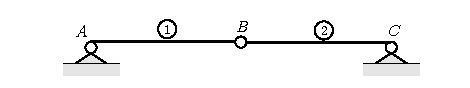
\includegraphics[scale=1.3]{figure/equilibrio/classificazione_deg}
\end{center}
Adesso abbiamo due travi e dunque $\mathscr{g}=6$; la molteplicità dei vincoli è $\mathscr{v}=2+2+2=6$, quindi $\mathscr{g}-\mathscr{v}=0=\mathscr{l}-\mathscr{i}$. Il sistema è isostatico o degenere. Cerchiamo di valutare la labilità, se presente.  Il centro di rotazione di 1 si troverebbe in $A$, mentre quello di 2 in $C$; il centro relativo invece sarebbe in $B$. Osserviamo che i tre centri sono allineati, quindi rispettano il primo teorema di Aronhold--Kennedy: il sistema ammette un cinematismo. Avendo determinato in maniera univoca i centri, allora $\mathscr{l}=1$ e dunque $\mathscr{i}=1$. Il sistema ha un vincolo sovrabbondante, ma inefficace ed è dunque degenere: il punto $B$ infatti può muoversi verticalmente e il vincolo sovrabbondante non è tale da impedirlo.

Concludiamo con un ultimo esempio
\begin{center}
	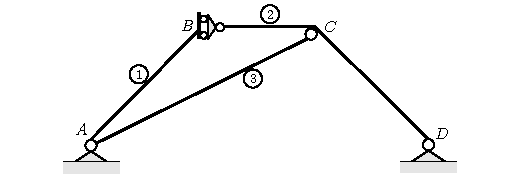
\includegraphics[scale=1.3]{figure/equilibrio/classificazione_es}
\end{center}
Il sistema adesso contempla 3 corpi e dunque $\mathscr{g}=9$. Per il calcolo della molteplicità dei vincoli occorre un po' di attenzione per quel che concerne la cerniera in $A$, dato che lì vi concorrono 2 travi e un vincolo esterno. Analizziamo il caso di due travi connesse tramite una cerniera, come nella figura sotto (sinistra).
\begin{center}
	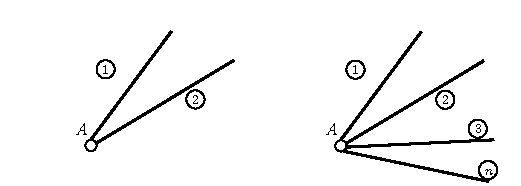
\includegraphics[scale=1.3]{figure/equilibrio/cerniera_travi}
\end{center}
La condizione di vincolo è
\begin{equation}
	\ub^{(1)}(\xb_{A})=	\ub^{(2)}(\xb_{A}),
	% \qquad	\ub^{(1)}(\xb_{A})=	\ub^{(3)} (\xb_{A})
\end{equation}
cui corrispondono due condizioni scalari:
\begin{equation}
\begin{aligned}
		&u_1^{(1)}(\xb_{A})=	u_1^{(2)},(\xb_{A})  \qquad 	u_2^{(1)}(\xb_{A})=	u_2^{(2)}(\xb_{A}),
		%\\	&u_1^{(1)}(\xb_{A})=	u_1^{(3)}(\xb_{A}), \qquad u_2^{(1)}(\xb_{A})=	u_2^{(3)}(\xb_{A}).
\end{aligned}
\end{equation}
Il vincolo ha dunque molteplicità 2. Se vi convergono tre travi, le condizioni scalari di vincolo diventano 
\begin{equation}
	\begin{aligned}
		&u_1^{(1)}(\xb_{A})=	u_1^{(2)}(\xb_{A}),  \qquad 	u_2^{(1)}(\xb_{A})=	u_2^{(2)}(\xb_{A}),
		\\	
		&u_1^{(1)}(\xb_{A})=	u_1^{(3)}(\xb_{A}), \qquad u_2^{(1)}(\xb_{A})=	u_2^{(3)}(\xb_{A}).
	\end{aligned}
\end{equation}
%
e dunque la molteplicità è 4. Se sulla cerniera convergono $n$ travi (come nella figura sopra a destra) le condizioni di vincolo sono $2(n-1)$.

Tornando all'esempio, nel punto $A$, oltre alle condizioni di vincolo interno tra le due travi appena descritto, è presente l'ulteriore condizione $\ub(\xb_{A})=\mathbf{0}$, cui corrispondono due condizioni scalari. Dunque, complessivamente, il vincolo in $A$ ha molteplicità 4. La molteplicità totale è allora $\mathscr{v}=4+1+2+2=9$. Essendo allora $\mathscr{g}-\mathscr{v}=0=\mathscr{l}-\mathscr{i}$, la struttura o è isostatica o è degenere. Cerchiamo di determinare la labilità. Se esistono, i centri del corpo 1 e 3 si trovano sulla cerniera in $A$, così come quello del corpo 2 si trova in $D$. Il centro relativo $C_{13}$ è sempre in $A$, il centro relativo $C_{23}$ è in $C$, violando il primo teorema di Aronhold--Kennedy per i corpi 2 e 3, che dunque non ammettono cinematismi. Il punto $B$ dunque non può muoversi e pertanto è come se fosse vincolato a terra; questa circostanza costringerebbe il centro di rotazione di 1 a trovarsi sull'asse del carrello, circostanza incompatibile con la richiesta già espressa che si trovi in $A$. Quindi neanche il corpo 1 ammette cinematismi e dunque $\mathscr{l}=0$. Il sistema  è allora isostatico.

\section{Equazione dei Lavori Virtuali}
Dell'equazione dei lavori virtuali, discussa nella Sez. \ref{ELV1D} nel caso monodimensionale  e nella Sez. \ref{ELV3Ds} nel caso tridimensionale, si può dare un'utile formulazione anche nel caso della teoria della trave. Partiamo dalla definizione di lavoro esterno e adattiamola a corpi a forma di trave, che abbiano una cinematica descritta da \eqref{u3d}, che ripetiamo qui per comodità del lettore:
	\begin{equation}\
	\hat\ub(\pb, z)=\ub(z)+\varthetab(z)\times\pb;
\end{equation}
ne segue che 
	\begin{equation}
\begin{aligned}
\Lc_e(\Tc)&=\int_{\Tc}\bb\cdot \hat\ub+\int_{\partial \Tc}\sb\cdot \hat\ub=\int_0^\ell\int_{\Sc}\big(\bb\cdot(\ub+\varthetab\times\pb)\big)+\int_0^\ell\int_{\partial\Sc}\sb\cdot(\ub+\varthetab\times\pb)\\
&+\int_{\Bc_0}\sb\cdot(\ub+\varthetab\times\pb)	+\int_{\Bc_\ell}\sb\cdot(\ub+\varthetab\times\pb)\\
&=\int_0^\ell(\qb\cdot \ub+\cb\cdot \varthetab)+\qb_0\cdot \ub(0)+\qb_\ell\cdot \ub(\ell)+\cb_0\cdot \varthetab(0)+\qb_\ell\cdot \varthetab(\ell),
\end{aligned}
\end{equation}
dove si è fatto uso delle definizioni \eqref{qb} e \eqref{qb} e dove
\begin{equation}
\qb_0\coloneqq\int_{\Bc_0}\sb, \qquad \qb_\ell\coloneqq\int_{\Bc_\ell}\sb, \qquad 
\cb_\ell\coloneqq\int_{\Bc_0}\pb\times\sb, \qquad \cb_\ell\coloneqq\int_{\Bc_\ell}\pb\times\sb,
\end{equation}
sono le forze e le coppie concentrate applicate agli estremi della trave.

Diciamo che il sistema di spostamenti e deformazioni $\{\ub, \varthetab; \eb, \kb\}$ è \textit{congruente} se

\begin{equation}\label{siscongr}
		\eb=\ub'-\varthetab\times \eb_3,  \qquad \kb=\varthetab'.
\end{equation}

Il sistema di  carichi e sforzi $\{\qb, \cb; \fb, \mb\}$ è \textit{equilibrato} (in assenza di carichi concentrate) se
\begin{equation}
\fb'+\qb =\mathbf{0}, \qquad \mb'+\eb_{3}\times \fb +\cb=\mathbf{0}.
\end{equation}

%Diciamo che il sistema di spostamenti e deformazioni $\{v_x, v_y, w, \varphi_x, \varphi_y, \vartheta_t; \gamma_x, \gamma_y, \varepsilon, \kappa_x, \kappa_y, \kappa_t\}$ è \textit{congruente} se 
%\begin{equation}
%\begin{aligned}
%	&\gamma_x=  v'_x-\varphi_y, \qquad &&\gamma_y= v'_y+\varphi_x, \qquad &&\kappa_t=\vartheta',\\
%	&	\varepsilon= w', \quad &&\kappa_x= \varphi_x', \quad  &&\kappa_y= \varphi_y',
%	\end{aligned}
%\end{equation}
%
%Il sistema di carichi e sforzi $\{ p_1, p_2, q, c_1, c_2, c_t; T_1, T_2, N, M_1, M_2, M_t\}$ è \textit{equilibrato} se
%	\begin{equation}
%\begin{aligned}
%&p_1(z)+T_1'(z)=0, \qquad && p_2(z)+T_2'(z)=0, \qquad && q(z)+N'(z)=0, \\
%&c_1(z)+M_1'(z)-T_2(z)=0, &&c_2(z)+M_2'(z)+T_1(z)=0, &&c_t(z)+M_t'(z)=0.
%\end{aligned}
%\end{equation}


Vale il seguente 
\begin{definition}
	\textbf{\textit{Teorema dei Lavori Virtuali}}. Sia $\{\ub, \varthetab; \eb, \kb\}$ un sistema di spostamenti e deformazioni congruenti e siano  $\{\qb, \cb; \fb, \mb\}$ un sistema di carichi e sforzi equilibrati. Allora il \textit{lavoro virtuale esterno}
	\begin{equation}
		\begin{aligned}
			\Lc_e(\Tc)=\int_0^\ell(\qb\cdot \ub+\cb\cdot \varthetab)+\qb_0\cdot \ub(0)+\qb_\ell\cdot \ub(\ell)+\cb_0\cdot \varthetab(0)+\qb_\ell\cdot \varthetab(\ell),
		\end{aligned}
	\end{equation}
	è uguale al lavoro \textit{virtuale interno }
	\begin{equation}
		\Lc_i(\Tc)=\int_{\Tc}\fb \cdot \eb + \mb \cdot \kb.
	\end{equation}
\end{definition}

La dimostrazione è analoga a quella già vista. Poiché $\{\qb, \cb; \fb, \mb\}$ sono equilibrati, possiamo scrivere 
	\begin{equation}
	\begin{aligned}
		\Lc_e(\Tc)=\int_0^\ell(-\fb'\cdot \ub-\mb'\cdot \varthetab-\eb_{3}\times \fb\cdot \varthetab)+\qb_0\cdot \ub(0)+\qb_\ell\cdot \ub(\ell)+\cb_0\cdot \varthetab(0)+\qb_\ell\cdot \varthetab(\ell).
	\end{aligned}
\end{equation}
Poiché
\begin{equation}
\begin{aligned}
&	\int_{0}^\ell\big(-\fb'\cdot\ub-\mb'\cdot \varthetab\big)=\int_{0}^\ell  \Big(-(\fb\cdot \ub)'+\fb\cdot\ub'-(\mb\cdot \varthetab)'+\mb \cdot\varthetab'\Big)\\
&=\int_{0}^\ell \Big(\fb\cdot\ub'+\mb \varthetab' \Big)+\fb(0)\cdot\ub(0)-\fb(\ell)\cdot\ub(\ell)+\mb (0)\cdot \varthetab(0)-\mb \cdot\varthetab(\ell),
\end{aligned}
\end{equation}
riconoscendo che
\begin{equation}
	\fb(0)=-\qb (0), \qquad \fb(\ell)=\qb (\ell), \qquad \mb (0)=-\cb(0), \qquad \mb (\ell)=\cb (0),
\end{equation}
concludiamo che
	\begin{equation}
	\begin{aligned}
		\Lc_e(\Tc)=\int_0^\ell\fb\cdot( \ub'-\varthetab\times\eb_3)+\mb\cdot \varthetab' ,
			\end{aligned}
\end{equation}
da cui, viste le \eqref{siscongr}, segue la tesi.

Supponiamo adesso che in $j$ punti della trave siano presenti delle forze concentrate $\qb_{oj}$ ($j=1,\ldots J$) e che in $k$ punti siano presenti delle coppie concentrate $\cb_{ok}$ ($k=1,\ldots K$). L'espressione del lavoro esterno può essere allora scritto come
\begin{definition}
	\begin{equation}
\Lc_e(\Tc)=\int_0^\ell(\qb\cdot \ub+\cb\cdot \varthetab)+\sum_{j=1}^{J}(\qb_{o}\cdot\ub)_j+\sum_{k=1}^{K}(\cb_{o}\cdot\varthetab)_k,
\end{equation}
\end{definition}
dove
\begin{equation}
(\qb_{o}\cdot\ub)_j\coloneqq \qb_{o}(z_j)\cdot \ub(z_j), \qquad (\cb_{o}\cdot\varthetab)_k\coloneqq \cb_{o}(z_k)\cdot \varthetab(z_k),
\end{equation}
rappresentano il lavoro compiuto dalla forza $j$-esima forza $\qb_{oj}$ e dalla $k$-esima forza $\qb_{ok}$ per lo spostamento $\ub(z_j)$ e la rotazione $\varthetab(z_k)$, rispettivamente. Le forze e le coppie concentrate agli estremi sono state inglobate nella sommatoria.
È facile verificare che il teorema continua ad essere valido, così come lo sono  le seguenti proposizioni, già discusse nel casi 1D e 3D, \textit{mutatis mutandis}:
\begin{definition}
	\begin{equation}
		\mathcal{L}_i=\mathcal{L}_e\quad\forall\{\eb, \kb; \ub, \varthetab\}\text{ congruenti}\quad\Longrightarrow\quad\{\fb, \mb; \qb, \cb \}\text{ equilibrati}
	\end{equation}
\end{definition}
e
\begin{definition}
	\begin{equation}
		\mathcal{L}_i=\mathcal{L}_e\quad\forall\{\fb, \mb; \qb, \cb\}\text{ equilibrati}\quad\Longrightarrow\quad\{\eb, \kb; \ub, \varthetab\}\text{ congruenti.}
	\end{equation}
\end{definition}
Le dimostrazioni sono banali adattamenti di quanto già discusso.


Nel caso di trave piana, utilizzando le componenti, si trova facilmente
\begin{definition}
	\begin{equation}
\Lc_e=\int_{0}^{\ell}(q w+ p v+ c\varphi)+ \sum_{i=1}^{I}(Q w)_i+\sum_{j=1}^{J}(P v)_j+\sum_{k=1}^{K}(C \varphi)_k,
\end{equation}
\end{definition}
con ovvio significato dei simboli, e
\begin{definition}
	\begin{equation}
\Lc_i=\int_{0}^{\ell}N \varepsilon+T\gamma+ M\kappa.
\end{equation}
\end{definition}

\subsection{Impieghi dell'equazione dei lavori virtuali}\label{ELVimp}
L'equazione dei lavori virtuali può essere convenientemente adoperata per calcolare speditamente spostamenti o rotazioni di singoli punti dell’asse o sezioni di una travatura, assegnate che siano le deformazioni.

Utilizziamo l'esempio sotto per spiegare come. Si supponga che la mensola $AB$ sia soggetta ad una deformazione flessionale assegnata $\bar{\kappa}>0$ e si supponga di voler determinare lo spostamento verticale del punto $B$.
\begin{center}
		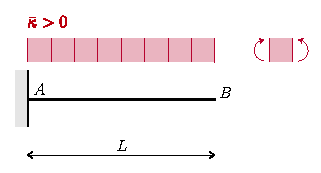
\includegraphics[scale=1.2]{figure/equilibrio/esempio6}
\end{center}

Per farlo abbiamo necessità di scegliere un sistema congruente ed uno equilibrato, generalmente distinti. Dato che cerchiamo uno spostamento nel sistema assegnato, scegliamo quello come sistema congruente; come sistema equilibrato ne scegliamo uno con una forza unitaria avente direzione e verso dello spostamento cercato, come indicato sotto. Al sistema equilibrato scelto corrispondono le caratteristiche della sollecitazione sotto rappresentate.
\begin{center}
	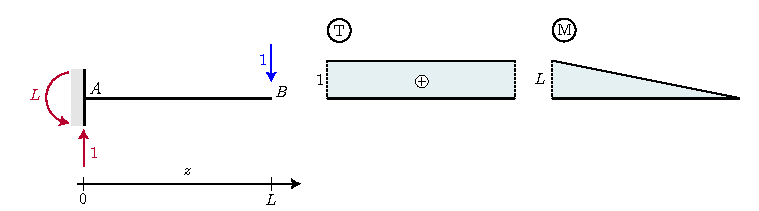
\includegraphics[scale=1.2]{figure/equilibrio/esempio6_1}
\end{center}

È immediato verificare che, scelta l'ascissa $z$ come in figura,
\begin{equation}
	T(z)=1, \qquad M(z)=z-L.
\end{equation}
 Possiamo a questo punto valutare il lavoro virtuale esterno, considerando i carichi del sistema equilibrato e gli spostamenti del sistema congruente. L'aggettivo virtuale è particolarmente pertinente, visto che tra i due sistemi non vi è alcun legame.
 Risulta allora:
 \begin{equation}
 \Lc_e=1\cdot v_B.
 \end{equation}
Il lavoro virtuale interno si determina considerando gli sforzi del sistema equilibrato e le deformazioni del sistema congruente:
\begin{equation}
\Lc_i=\int_0^L M(z)\bar{\kappa}=\bar{\kappa}\int_0^L (L-z)=-\frac{1}{2}\bar{\kappa}L^2.
\end{equation}
Richiedendo che i due lavori siano eguali, determiniamo lo spostamento cercato:
\begin{equation}
v_B=-\frac{1}{2}\bar{\kappa}L^2.
\end{equation}
La circostanza che $v_B$ sia negativo indica che il punto $B$ si sposta nella direzione opposta alla forza unitaria applicata nel sistema equilibrato, e dunque verso l'alto, come ci si attende.

Supponiamo adesso di voler determinare la rotazione della sezione in $B$. Scegliamo allora come sistema equilibrato quello sotto, in cui applichiamo una coppia unitaria nella direzione e nel verso dello spostamento cercato.

\begin{center}
	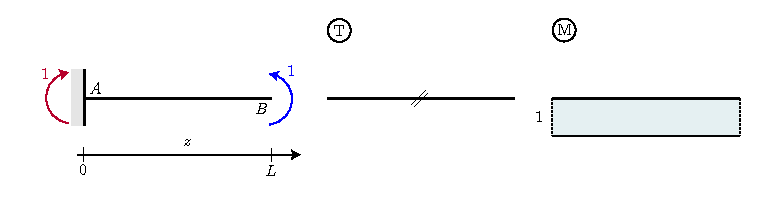
\includegraphics[scale=1.2]{figure/equilibrio/esempio6_2}
\end{center}
 In questo caso
 \begin{equation}
 	T(z)=0, \qquad M(z)=1.
 \end{equation}
 
 Il lavoro virtuale esterno risulta adesso
\begin{equation}
\Lc_e=1\cdot \varphi_B,
\end{equation}
mentre il lavoro virtuale interno è
\begin{equation}
\Lc_i=\int_0^LM(z)\bar{\kappa}=\bar{\kappa}L,
\end{equation}
donde
\begin{equation}
\varphi_B=\bar{\kappa}L.
\end{equation}
Il segno positivo sta a significare che la sezione ruota nello stesso verso della coppia applicata nel sistema equilibrato, e dunque in senso antiorario.



